\documentclass[11pt,a4paper,oneside]{article}

% -------------------------------------------------
% Basic packages
% -------------------------------------------------
\usepackage[T1]{fontenc}
\usepackage[utf8]{inputenc}
\usepackage[english]{babel}
\usepackage{lmodern}
\usepackage{microtype}
\usepackage[a4paper,margin=1.18in,headheight=15pt]{geometry}
\usepackage{amsmath,amssymb,amsfonts,amsthm,mathtools}
\usepackage{bm}
\usepackage{enumitem}
\usepackage{booktabs}
\usepackage{array}
\usepackage{xcolor}
\usepackage{graphicx}
\usepackage{caption}
\usepackage{hyperref}
\usepackage{setspace}
\usepackage{fancyhdr}
\usepackage{titlesec}
\usepackage[most]{tcolorbox}
\usepackage{placeins}
\usepackage[capitalize,noabbrev]{cleveref}

\hypersetup{
  colorlinks=true,
  linkcolor=blue!50!black,
  citecolor=red!55!black,
  urlcolor=teal!60!black,
  pdftitle={Integrated Multiresolution Analysis and Academic Performance System},
  pdfauthor={Cesar Galindo Lopez and Gabriel Villafuerte C.}
}

\theoremstyle{definition}
\newtheorem{definition}{Definition}[section]
\newtheorem{remark}[definition]{Remark}

\definecolor{ihesblue}{RGB}{25,62,114}
\definecolor{ihesgold}{RGB}{160,120,40}
\pagestyle{fancy}
\fancyhf{}
\fancyhead[L]{\textsc{Wavelet-based sentiment}}
\fancyhead[R]{\textsc{Galindo L\'opez \& Villafuerte C.}}
\fancyfoot[C]{\thepage}
\renewcommand{\headrulewidth}{0.35pt}
\renewcommand{\footrulewidth}{0pt}
\titleformat{\section}{\Large\bfseries\color{ihesblue}}{\thesection.}{0.65em}{}
\titleformat{\subsection}{\large\bfseries\color{ihesblue}}{\thesubsection.}{0.65em}{}
\titlespacing*{\section}{0pt}{1.9em}{1.05em}
\titlespacing*{\subsection}{0pt}{1.45em}{0.95em}
\tcbset{colback=white,colframe=ihesblue!65!black,boxrule=0.5pt,arc=1.5pt}
\setlength{\parskip}{0.85em}
\setstretch{1.13}
\setlength{\parindent}{0pt}
\captionsetup{font=small,labelfont=bf,labelsep=period}

\newtcolorbox{ideaBox}[1][]{enhanced,breakable,colback=blue!2,colframe=ihesblue,
  borderline west={1.5pt}{0pt}{ihesblue},title=Key idea,fonttitle=\bfseries,#1}
\newtcolorbox{summaryBox}[1][]{enhanced,breakable,colback=gray!4,colframe=black!55,
  borderline west={1.5pt}{0pt}{black!70},title=Key formulas,fonttitle=\bfseries,#1}
\newtcolorbox{warningBox}[1][]{enhanced,breakable,colback=red!2,colframe=red!55!black,
  borderline west={1.5pt}{0pt}{red!75!black},title=Scope and limitations,fonttitle=\bfseries,#1}
\newtcolorbox{implBox}[1][]{enhanced,breakable,
  colback=violet!3!white,colframe=violet!50!black,
  borderline west={2pt}{0pt}{violet!65!black},
  title=Implementation,fonttitle=\bfseries\color{violet!80!black},
  attach boxed title to top left={yshift=-2mm,xshift=4mm},
  boxed title style={colback=violet!12,colframe=violet!50!black,boxrule=0.5pt},#1}

\title{\vspace{-1.5cm}\textbf{\Large Integrated Multiresolution Analysis and Academic Performance System}\\[2pt]
\large A sentiment index with an explicit statistical check of its efficiency --and of its limits--, via embeddings and the wavelet transform}
\author{C\'esar Galindo L\'opez \\ \small Universidad Panamericana \textperiodcentered\ Facultad de Empresariales, Ciudad UP
  \and Gabriel Villafuerte C. \\ \small \href{https://github.com/Gabriel44svg}{github.com/Gabriel44svg}}
\date{\small 2026}

\begin{document}
\maketitle

\begin{abstract}
\noindent We present a system that combines the quantitative signal of a course (grades,
midterms, risk status) with the qualitative signal of an open-ended feedback survey, producing
for the latter a per-student sentiment index $\hat\theta\in(-1,1)$: each response is turned into
a scalar signal indexed by token position (projecting each word's contextual embedding onto the
sentence embedding), which is decomposed with the discrete wavelet transform (DWT) into a
global-trend component and a local-fluctuation component. We accompany $\hat\theta$ with an
explicit statistical check --Fisher information and the Cram\'er--Rao bound under Gaussian and
Laplacian models-- and show, with simulations, exactly what that check certifies and what it
does not. We do not report runs on real course data: this is a methods article, accompanied by
illustrative simulations explicitly labeled as such, not a case study.

\medskip
\noindent\textbf{Keywords:} academic analytics, early warning, sentiment analysis, wavelet
transform, Fisher information, Cram\'er--Rao bound.
\end{abstract}

\begin{table}[h]
\centering
\small
\begin{tabular}{@{}p{0.42\linewidth}p{0.5\linewidth}@{}}
\toprule
\textbf{Code metadata} & \textbf{Value} \\
\midrule
Current code version & v1.0 \\
Permanent link to code/repository used for this code version &
  \href{https://github.com/Gabriel44svg/Galindo-C.-J.-y-Villafuerte-C.-G.-2026-.-SIAMDA}{github.com/Gabriel44svg/\ldots-SIAMDA} \\
Legal code license & MIT \\
Code versioning system used & git \\
Software code languages, tools, and services used &
  Python~3.11; Streamlit; sentence-transformers; PyWavelets; SciPy; pandas; Plotly; pytest \\
Compilation requirements, operating environments and dependencies &
  Python $\ge 3.10$; see \texttt{requirements.txt} (runtime) and \texttt{requirements-dev.txt}
  (tests) \\
Link to developer documentation/manual &
  \texttt{README.md} in the repository \\
Support email for questions & \texttt{jcgalindo@up.edu.mx} \\
\bottomrule
\end{tabular}
\caption{Code metadata (standard software-paper format).}
\label{tab:metadata}
\end{table}

\section{Motivation and significance}
\label{sec:motivacion}

A course generates two kinds of signal about a student's performance: a \emph{quantitative} one
(midterm grades, homework, presentations) and a \emph{qualitative} one (what the student writes
in an open-ended feedback survey). The quantitative signal is the one normally used to detect
academic risk; the qualitative one tends to be read impressionistically, with no metric. This
work proposes a metric for the second signal and asks whether it adds information about academic
risk beyond the first, via its empirical correlation with the final grade.

The construction of $\hat\theta$ combines two ingredients that are well established separately:
contextual sentence \emph{embeddings} obtained with Siamese-BERT-style networks
\cite{ReimersGurevych2019}, and the discrete wavelet transform as a multiresolution
signal-analysis tool \cite{Mallat1989}. What the system adds is an explicit statistical
validation layer for the group's aggregate sentiment estimator, grounded in the classical theory
of estimator efficiency \cite{Fisher1922,Rao1945,Cramer1946}, complemented by a normality test
\cite{ShapiroWilk1965} and a resampling variance estimate \cite{Efron1979}. The contribution of
this article is not any of those ingredients on its own, but documenting precisely what their
combination certifies --and, above all, what it does \emph{not} certify--, something the first
version of our own implementation stated imprecisely (\cref{sec:crb}).

\section{Software description}
\label{sec:descripcion}

\subsection{Software architecture}
\label{sec:arquitectura}

The system is organized into four modules:

\begin{enumerate}[leftmargin=1.4em]
  \item \textbf{Ingestion and normalization} (\texttt{datos.py}): reading grade files
  (CSV/Excel) with automatic column detection (student ID, name, midterms
  \texttt{E1,E2,\dots}, weighted exam score, homework, presentations, validation), handling of
  mixed text in non-numeric cells (\emph{``retake the final''}, \emph{``on academic
  reinstatement''}, \emph{``withdrew''}, etc.), and computation of a binary risk flag.
  \item \textbf{NLP and wavelet extraction} (\texttt{nlp\_wavelet.py}): sentence- and
  token-level embeddings (multilingual \emph{sentence-transformers}) over the survey's
  open-ended responses, and multiresolution decomposition of the resulting positional signal
  via DWT.
  \item \textbf{Theoretical validation} (\texttt{cramer\_rao.py}): Fisher information and the
  Cram\'er--Rao bound for the aggregate sentiment index, under Gaussian and Laplacian models,
  plus a normality test (Shapiro--Wilk) and a bootstrap estimate of the estimator's variance.
  \item \textbf{Interactive visualization}: a Streamlit interface with pages for data loading,
  course metrics, sentiment analysis, and theoretical validation, with automatic natural-language
  interpretations for each metric.
\end{enumerate}

\subsection{Software functionalities}
\label{sec:funcionalidades}

\subsubsection{Academic risk flag}

Let $c_i$ be student $i$'s final grade and $e_i\in\{\text{Normal},\ldots\}$ their validation
status (reinstatement, final exam, withdrawal, etc.). The system defines
\[
r_i = \mathbf{1}\{c_i < 70\} \ \vee\ \mathbf{1}\{e_i \neq \text{Normal}\},
\]
i.e., a student is flagged at risk if their grade falls below the passing threshold (70) or if
they have a special status on record, regardless of the numeric grade.

\subsubsection{Wavelet-based sentiment index}
\label{sec:indice}

For each student $i$, the multilingual \emph{sentence-transformers} model
(\texttt{paraphrase-multilingual-MiniLM-L12-v2}, dimension $d=384$) \cite{ReimersGurevych2019}
produces, in a single \emph{forward pass}: the sentence embedding $x_i\in\mathbb{R}^d$
(normalized to unit norm) and, for each token $t=1,\ldots,L_i$ of the response, a contextual
embedding $u_{i,t}\in\mathbb{R}^d$. From these a scalar signal is built, \emph{indexed by token
position in the text} --an axis with genuine temporal adjacency, unlike the embedding's
coordinates--, by projecting each token onto the response's overall semantic direction:
\[
s_i(t) \;=\; \langle u_{i,t},\, x_i\rangle, \qquad t=1,\ldots,L_i.
\]
The discrete wavelet transform \cite{Mallat1989} is applied to this 1D signal, with the
Daubechies-4 family and a default decomposition level $J=3$, bounded in practice by
$\min_i \texttt{pywt.dwt\_max\_level}(L_i,\text{wavelet})$ --the shortest response in the batch,
not a fixed dimension--:
\[
\mathrm{wavedec}(s_i, J) = \big(c^{(i)}_A,\ c^{(i)}_{D,1},\ \ldots,\ c^{(i)}_{D,J}\big),
\]
where $c^{(i)}_A$ are the approximation coefficients (the response's global trend, low frequency
\emph{in position}) and $c^{(i)}_{D,j}$ the detail coefficients at level $j$ (local
word-to-word fluctuation, high frequency). The energies are defined as
\[
E^{\mathrm{apr}}_i = \big\lVert c^{(i)}_A \big\rVert_2^2,
\qquad
E^{\mathrm{det}}_i = \sum_{j=1}^{J} \big\lVert c^{(i)}_{D,j} \big\rVert_2^2 ,
\]
and student $i$'s sentiment index is defined as
\[
\hat\theta_i \;=\; \tanh\!\left(\frac{E^{\mathrm{det}}_i - E^{\mathrm{apr}}_i}
{E^{\mathrm{det}}_i + E^{\mathrm{apr}}_i + \varepsilon}\right), \qquad \varepsilon = 10^{-9},
\]
so that $\hat\theta_i\in(-1,1)$: values close to $-1$ indicate energy concentrated in the
approximation (a contextual response, little local fluctuation) and values close to $+1$
indicate energy concentrated in the details (high local variability, interpreted here as
localized emotional charge).

\begin{implBox}[title=Design fix]
In an earlier version of this pipeline, the DWT was applied directly to the $384$ coordinates of
$x_i$, treating them as if they were a temporal signal. Those coordinates are axes of a learned
feature space with no intrinsic ordering or adjacency: permuting them does not change the
meaning of the text, but it did change $E^{\mathrm{apr}}_i$ and $E^{\mathrm{det}}_i$ under that
version, so the reading ``approximation = stable content, detail = emotion'' was not justified
by the transform's own mathematics. The formulation above --projecting each token onto the
sentence embedding and applying the DWT over \emph{token position}-- uses an axis with genuine
sequential structure, for which the DWT's split into global trend (approximation) and local
fluctuation (detail) does have the usual backing of wavelet theory \cite{Mallat1989}. Code:
\texttt{processing/nlp\_wavelet.py} (\texttt{obtener\_embeddings\_token},
\texttt{se\~nal\_por\_posicion}, \texttt{aplicar\_dwt\_posicional}).

An intermediate version of \texttt{obtener\_embeddings\_token} --after the fix above-- did build
the positional signal as described here, but called \texttt{modelo.encode()} \emph{twice} (once
for the sentence embedding, once for the token embeddings), i.e.\ two \emph{forward passes},
while the docstring and an earlier version of this paragraph claimed both outputs came from ``a
single forward pass''. Both statements were true individually and false together. The current
version uses a single call with \texttt{output\_value=None}, which sentence-transformers
documents as the way to obtain all outputs (including \texttt{sentence\_embedding} and
\texttt{token\_embeddings}) from one \emph{forward pass}, making the claim above true.
\end{implBox}

\subsubsection{Statistical validation: Fisher information and the Cram\'er--Rao bound}
\label{sec:crb}

Let $\hat\theta = (\hat\theta_1,\ldots,\hat\theta_N)$ be the group's sample of sentiment indices
(the data, not individual estimators of anything), treated as $N$ i.i.d.\ observations from a
distribution with location parameter $\mu$ (the group's average sentiment), and
$\bar\theta = \frac1N\sum_i \hat\theta_i$ the sample-mean estimator of $\mu$. The Cram\'er--Rao
bound \cite{Fisher1922,Rao1945,Cramer1946} lower-bounds the variance of any unbiased estimator of
$\mu$:
\[
\mathrm{Var}(\bar\theta) \;\ge\; \frac{1}{F(\mu)},
\qquad
F(\mu) = -\,\mathbb{E}\!\left[\frac{\partial^2}{\partial\mu^2}\ln p(X;\mu)\right],
\]
where $X=(\hat\theta_1,\ldots,\hat\theta_N)$ denotes the full sample (so
$p(X;\mu)=\prod_i p(\hat\theta_i;\mu)$ and $F(\mu)$ already incorporates the factor $N$, as in
the explicit formulas below).

\begin{summaryBox}
\textbf{Gaussian model.} Under $\theta\sim\mathcal N(\mu,\sigma^2)$, with
$\hat\mu=\bar\theta$ and $\hat\sigma^2$ the unbiased sample variance:
\[
F(\mu) = \frac{N}{\hat\sigma^2}, \qquad
\mathrm{CRB}_\mu = \frac{1}{F(\mu)} = \frac{\hat\sigma^2}{N}.
\]
\textbf{Laplacian model.} Under $\theta\sim\mathrm{Laplace}(\mu,b)$, with
$\hat\mu=\mathrm{median}(\hat\theta)$ and $\hat b = \frac1N\sum_i |\hat\theta_i-\hat\mu|$:
\[
F(\mu) = \frac{N}{\hat b^2}, \qquad
\mathrm{CRB}_\mu = \frac{\hat b^2}{N}.
\]
Unlike the Gaussian case, where the sample mean attains the bound \emph{exactly} for every $N$,
the sample median is the MLE of $\mu$ under the Laplacian model and only attains the bound
\emph{asymptotically} ($N\to\infty$); for finite $N$ its variance can exceed $\mathrm{CRB}_\mu$.
\textbf{Empirical estimator efficiency (EEE).} With $\widehat{\mathrm{Var}}(\bar\theta)$
estimated by \emph{bootstrap} \cite{Efron1979} ($B=500$ resamples with replacement):
\[
\mathrm{EEE} = \min\!\left(\frac{\mathrm{CRB}_\mu}{\widehat{\mathrm{Var}}(\bar\theta)},\ 1\right).
\]
\end{summaryBox}

The system complements this computation with a Shapiro--Wilk normality test \cite{ShapiroWilk1965}
on $\hat\theta$: if the resulting $p$-value is below $0.05$, the Laplacian model (more robust to
heavy tails) is recommended over the Gaussian one, using the sample median --the optimal
estimator under that model-- instead of the mean.

\begin{remark}
The Cram\'er--Rao bound certifies something precise and limited: how close the \emph{sample
mean} of $\hat\theta$ is to being an optimal estimator of itself under an assumed parametric
model. It does not certify that $\hat\theta$ correctly measures ``real sentiment'', nor does it
substitute for external validation (e.g.\ against human annotation) of the index.
\end{remark}

\begin{warningBox}[title=Gap: what this check does NOT certify]
Under the Gaussian model with unknown $\sigma^2$ estimated by $\hat\sigma^2$, the sample mean is
the minimum-variance unbiased estimator of $\mu$ \emph{for every} $N$ (Lehmann--Scheff\'e), with
$\mathrm{Var}(\bar\theta)=\sigma^2/N$ exactly. That is, under that model the efficiency is $1$ by
construction, not by merit of the NLP--wavelet pipeline: no alternative estimator of $\mu$ could
ever beat the sample mean. The comparison the system makes --$\mathrm{CRB}_\mu=\hat\sigma^2/N$
against $\widehat{\mathrm{Var}}(\bar\theta)$ estimated by \emph{bootstrap on the same sample}--
is, in the large-$N$ limit, a comparison between two ways of estimating the \emph{same} quantity
($\sigma^2/N$) from the \emph{same} data: the plug-in normal formula with $\hat\sigma^2$, and
resampling. That the two agree (EEE $\approx 1$) is therefore, to a large extent, a numerical
consistency check between bootstrap and the asymptotic formula for the variance of the mean
--something that happens for almost any reasonably large sample, regardless of how well the
embedding-and-wavelet pipeline captures actual sentiment--, and is \emph{not} evidence that the
NLP-wavelet pipeline extracts the maximum information available in the text. Verifying that
would require comparing $\hat\theta$ against an alternative feature-extraction pipeline (or
against human annotation) on the same text, not merely checking that the sample mean of
$\hat\theta$ is a good estimator of itself. \Cref{sec:resultados} illustrates this numerically:
in the simulation, $\mathrm{EEE}=100\%$ even though $\hat\theta$ \emph{rejects} normality
(Shapiro--Wilk $p<10^{-3}$). The interface's interpretive text
(\texttt{interpretar\_crb} in \texttt{interpretacion.py}, and the ``Theoretical framework'' in
\texttt{validacion.py}) used to overclaim exactly this and has since been corrected to reflect
the check's actual scope.
\end{warningBox}

\subsubsection{Correlation with academic performance}

As the final step of the analysis, the system computes the Pearson correlation coefficient $r$
\cite{Pearson1896} between $\hat\theta_i$ and each student's grade $c_i$, together with its
associated $p$-value and sample size $N$. A significant negative correlation ($r<0$, $p<0.05$) is
interpreted as evidence that higher emotional charge in the responses is associated with lower
performance; a significant positive correlation is interpreted as possible extrinsic motivation.
The system classifies the strength of the association using thresholds ($|r|\ge 0.6$ strong,
$|r|\ge 0.3$ moderate, $|r|<0.3$ weak) and explicitly reports when the correlation is not
significant, without forcing a risk narrative where there is no statistical evidence.

\section{Illustrative example}
\label{sec:resultados}

\begin{warningBox}[title={These figures are simulation, not course data}]
No real student data was used to generate this section. The signals, embeddings, and grades are
synthetic, built to exercise the real code in \texttt{processing/nlp\_wavelet.py} and
\texttt{processing/cramer\_rao.py} --the same functions the application uses-- on controlled
inputs, for the sole purpose of showing how to read the plots the system produces and of
numerically exhibiting the point made in \cref{sec:crb}. The correlation in
\cref{fig:correlacion} is imposed by construction in the simulation, not observed. Generation
code: \texttt{generar\_figuras\_articulo\_en.py}.
\end{warningBox}

We simulate $N=60$ responses of variable length ($L_i$ a uniform integer in $\{12,\ldots,54\}$
tokens), each with an ``emotional intensity'' $e_i\sim\mathrm{Gamma}(2,\,0.5)$ that controls the
amplitude of local bursts inserted into a random-walk trend (\cref{fig:señal}), and a simulated
grade $c_i = \mathrm{clip}(92 - 9\,e_i + \eta_i,\,40,\,100)$ with $\eta_i\sim\mathcal N(0,6^2)$,
to illustrate how to read a negative correlation.

\begin{figure}[htb]
\centering
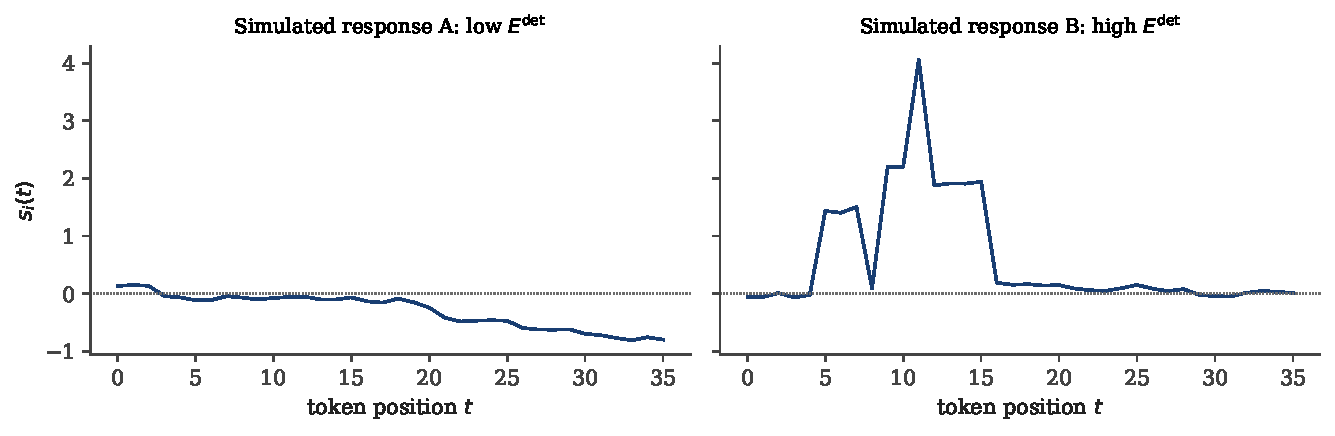
\includegraphics[width=0.92\linewidth]{figs_en/fig_signal_example.pdf}
\caption{Two simulated positional signals $s_i(t)$: one with low imposed emotional intensity
(left) and one with marked local bursts (right), producing low and high $E^{\mathrm{det}}$
respectively.}
\label{fig:señal}
\end{figure}

\begin{figure}[htb]
\centering
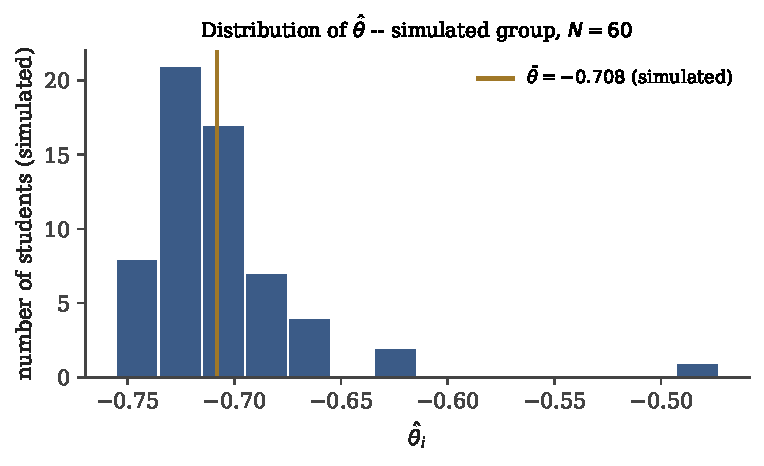
\includegraphics[width=0.75\linewidth]{figs_en/fig_theta_hist.pdf}
\caption{Distribution of $\hat\theta$ over the simulated group ($N=60$). The visible asymmetry
is consistent with the rejection of normality reported in the text (Shapiro--Wilk $p<10^{-3}$).}
\label{fig:theta_hist}
\end{figure}

\begin{figure}[htb]
\centering
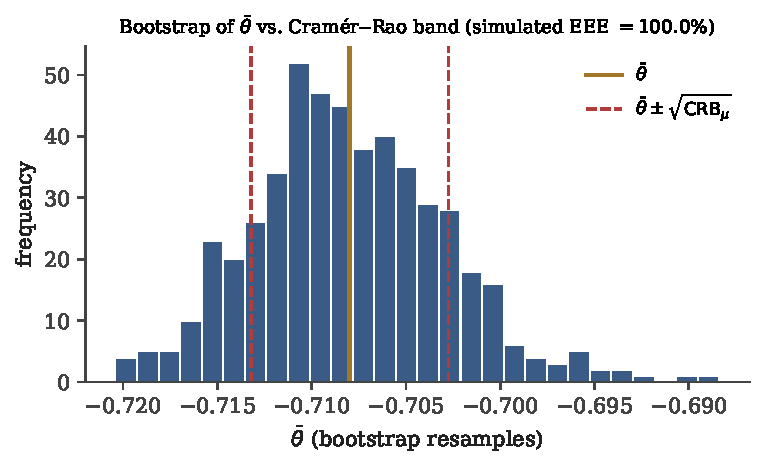
\includegraphics[width=0.75\linewidth]{figs_en/fig_bootstrap_crb.pdf}
\caption{Bootstrap distribution of $\bar\theta$ ($B=500$) against the
$\bar\theta\pm\sqrt{\mathrm{CRB}_\mu}$ band. In this simulation $\mathrm{EEE}=100\%$
\emph{even though} $\hat\theta$ rejects normality --the central point of \cref{sec:crb}: this
figure does not measure whether the pipeline extracts information from the text.}
\label{fig:bootstrap}
\end{figure}

\begin{figure}[htb]
\centering
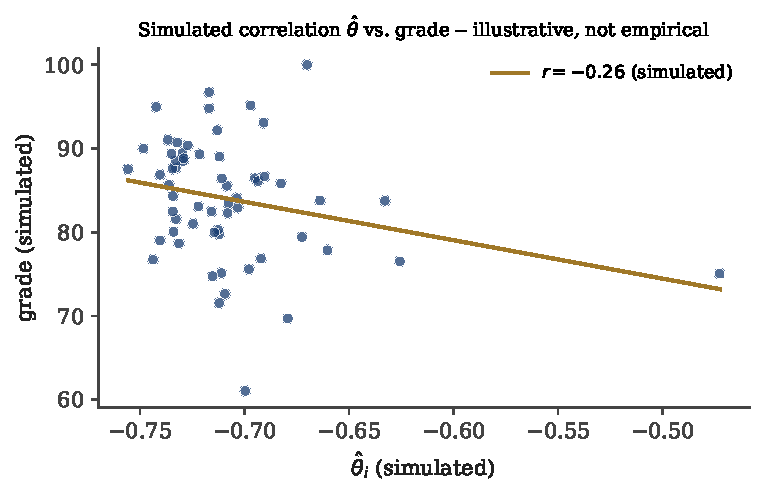
\includegraphics[width=0.75\linewidth]{figs_en/fig_correlation.pdf}
\caption{Simulated correlation between $\hat\theta$ and the grade, imposed by construction
($c_i$ was defined as a decreasing function of the simulated emotional intensity $e_i$) to
illustrate how this plot is read in the real interface.}
\label{fig:correlacion}
\end{figure}

\FloatBarrier

\section{Impact}
\label{sec:impacto}

The system targets a generic teaching problem (not specific to one course or institution): the
qualitative signal from an open-ended feedback survey is rarely analyzed with the same rigor as
the quantitative signal from grades, despite being available in practically any course. By
packaging token embeddings, DWT, and a Fisher/Cram\'er--Rao check into a reproducible pipeline
with an interactive interface, the system lowers the barrier for an instructor without training
in NLP or estimation theory to produce --and, above all, \emph{correctly interpret}-- a
per-group aggregate sentiment index, including when \emph{not} to trust it. That last part is,
in practice, the least common component in similar tools: most educational-analytics dashboards
report a number without stating what it mathematically guarantees and what it does not.

The honest limit on immediate reuse is the one already documented in the previous sections: the
index $\hat\theta$ depends on the chosen embedding model, on the wavelet family and level, and on
the survey's size; with $N<30$ the bootstrap variance estimates are unstable, and the system
itself warns about this in the interface. The textual interpretations generated by the
\texttt{interpretacion.py} module are reading suggestions, not definitive conclusions, and should
be checked against the instructor's judgment and, when warranted, institutional
psycho-pedagogical support. As documented in \cref{sec:crb}, the Cram\'er--Rao check certifies
the statistical coherence of $\bar\theta$ under the assumed model, not the quality of
$\hat\theta$ as a measure of sentiment; that second question --the one that would actually matter
for justifying institutional adoption-- remains open and would require external comparison
(human annotation, or another extraction pipeline) on real course data, which this article
deliberately does not report. Until that validation exists, responsible reuse of the system is
as an exploratory, supportive tool, not as the sole basis for a decision about a student.

\begin{implBox}[title=Reuse]
Code, sample data, 22 automated tests (\texttt{pytest}, run in CI on every \emph{push}), and an
MIT license are at
\href{https://github.com/Gabriel44svg/Galindo-C.-J.-y-Villafuerte-C.-G.-2026-.-SIAMDA}{github.com/Gabriel44svg/\ldots-SIAMDA}
(see also \cref{tab:metadata}). Architecture and dependency details are in \cref{sec:arquitectura}.
\end{implBox}

\section{Conclusions}

This system integrates two signals from a course --grades and open-ended survey responses--
under one dashboard, and adds to the latter a reproducible metric ($\hat\theta$, via token
embeddings, positional projection, and DWT) together with a statistical check of the coherence
of its aggregate mean (Fisher information and the Cram\'er--Rao bound, under Gaussian and
Laplacian models). The result is an early-warning system that makes the link between a group's
tone and its performance explicit rather than impressionistic, and that honestly documents what
its statistical layer certifies and what it does not. Validating $\hat\theta$ against human
annotation on real course data remains as future work.

\section*{Declaration of competing interest}

The authors declare that they have no known competing financial interests or personal
relationships that could have appeared to influence the work reported in this paper.

\begin{thebibliography}{9}

\bibitem{Fisher1922} R.~A.~Fisher, \emph{On the mathematical foundations of theoretical
statistics}, Philos. Trans. R. Soc. Lond. A \textbf{222} (1922), 309--368.

\bibitem{Rao1945} C.~R.~Rao, \emph{Information and the accuracy attainable in the estimation of
statistical parameters}, Bull. Calcutta Math. Soc. \textbf{37} (1945), 81--91.

\bibitem{Cramer1946} H.~Cram\'er, \emph{Mathematical Methods of Statistics}, Princeton University
Press, 1946.

\bibitem{ShapiroWilk1965} S.~S.~Shapiro and M.~B.~Wilk, \emph{An analysis of variance test for
normality (complete samples)}, Biometrika \textbf{52} (1965), no.~3/4, 591--611.

\bibitem{Efron1979} B.~Efron, \emph{Bootstrap methods: another look at the jackknife}, Ann.
Statist. \textbf{7} (1979), no.~1, 1--26.

\bibitem{Pearson1896} K.~Pearson, \emph{Mathematical contributions to the theory of evolution.
III. Regression, heredity, and panmixia}, Philos. Trans. R. Soc. Lond. A \textbf{187} (1896),
253--318.

\bibitem{Mallat1989} S.~G.~Mallat, \emph{A theory for multiresolution signal decomposition: the
wavelet representation}, IEEE Trans. Pattern Anal. Mach. Intell. \textbf{11} (1989), no.~7,
674--693.

\bibitem{ReimersGurevych2019} N.~Reimers and I.~Gurevych, \emph{Sentence-BERT: sentence
embeddings using Siamese BERT-networks}, in Proc.\ 2019 Conf.\ Empirical Methods in Natural
Language Processing (EMNLP-IJCNLP), Hong Kong, 2019, pp.~3982--3992.

\end{thebibliography}

\end{document}
